\documentclass[10pt,a5paper]{article}
\renewcommand{\baselinestretch}{1.0}
\usepackage{cite}
\usepackage[dvips]{graphicx}
\usepackage{psfrag}
\usepackage{color}
\usepackage[cmex10]{amsmath}
\usepackage{amsfonts}
\usepackage[font=footnotesize, captionskip=10pt]{subfig}
\usepackage{tikz}
\usepackage{flushend}
\usepackage{times}
\usepackage[margin=1.5cm]{geometry}

\usepackage[slovak]{babel}
\usepackage[utf8]{inputenc}
\usepackage[T1]{fontenc}

\pagestyle{empty}

\hyphenation{net-works}
\newtheorem{remark}{Remark}

\begin{document}

\title{Function aproximation using experimental artifical neuron model}
\author{Michal Chovanec\\ Lukáš Čechovič \\
michal.chovanec@fri.uniza.sk, lukas.cechovic@fri.uniza.sk}
\date{}
\maketitle
\thispagestyle{empty}

%\noindent$^1$\ affiliation\\
%\noindent$^2$\ affiliation\\

\noindent {\bf Keywords:} neural network, approximation, neuron model, McCulloch Pitts neuron

\noindent {\bf Abstract:} In this paper we introduce experimental neuron model,
using inputs signal's multiplications. Some approximation abilities test's were done
and further applications introduced.

\section{Introduction}

Feed forward neural network can be used for approximation of any continuous function \cite{bib:Approximation_1}, \cite{bib:Approximation_2}, \cite{bib:Approximation_3}
Some problems are also know \cite{bib:Approximation_problem_1} - using of many neuons, or layers -
which is serious problem for real time applications \cite{bib:Approximation_problem_2}, especially
real time control, robotics, image recognition or virtual agents. Other problem is gradient backpropagation
which can stay in local minima \cite{bib:Backpopagation_01}. Some techniques, like momentum can help in this problem,
or stochastic optimization algorithms.

Some common neural network applications \cite{bib:NN_Applications_01} can be found in :

\begin{itemize}
  \item Stock Market Prediction
  \item Medical Diagnosis
  \item Process Control
  \item Prediction
  \item Classification
  \item Change and Deviation Detection
  \item Knowledge Discovery
  \item Response Modeling
  \item Time Series Analysis
  \item Staff Scheduling
  \item Personnel Profiling
\end{itemize}

To reduce neurons and layers count we modify neuron model to multiplication ability.


\section{Preceding experimets}

Common used neuron McCulloch-Pitts \ref{eq:McCulloch_Pitts}.

\begin{equation}
\label{eq:McCulloch_Pitts}
  y(n) = \varphi(\sum_{i = 0}^{N-1} x_i(n)w_i(n))
\end{equation}

where \\
$x(n)$ is input vector \\
$w(n)$ is weight vector \\
$y(n)$ is neuron output \\
and $\varphi(g)$ is activation function \\

Common used activation function are sigmoid, tahn, linear, rectifier, and step functions
are on \ref{img:activation_functions}.


\begin{figure}[!ht]
\centering
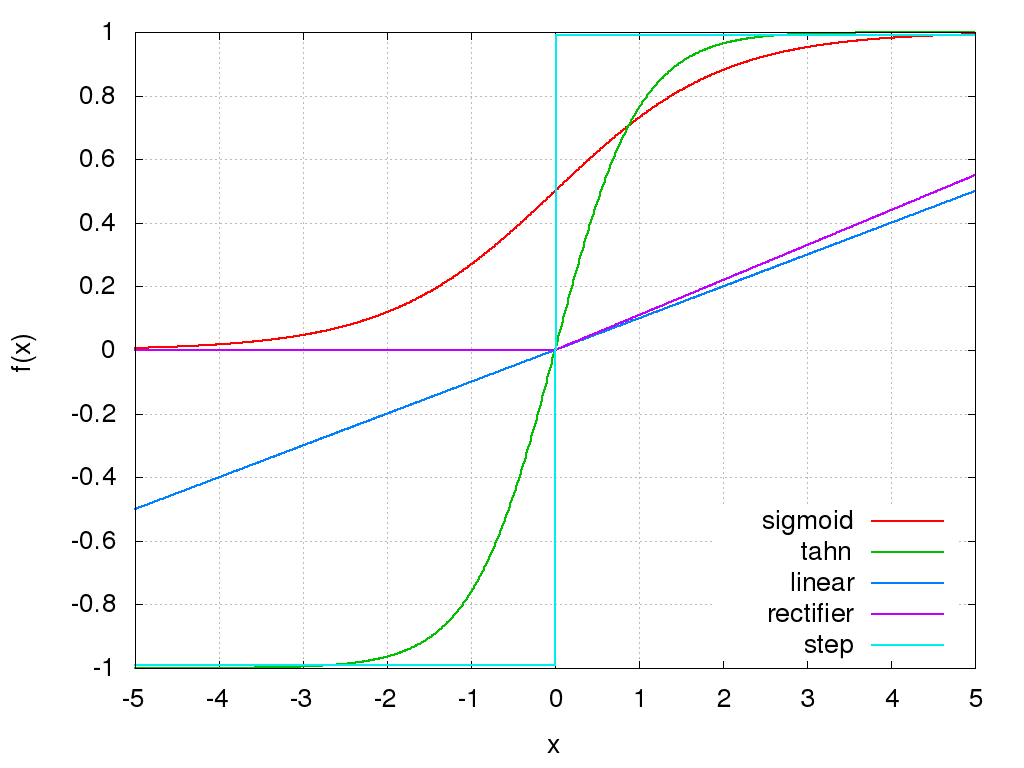
\includegraphics[width=3.0in]{images/nn_functions.png}
\caption{Activation functions}
\label{img:activation_functions}
\end{figure}

Consider following problem : We need to approximate multiplexer function with inputs
$A$ $B$ and select $S$ (figure )\ref{img:multiplexer}).

\begin{figure}[!ht]
\centering
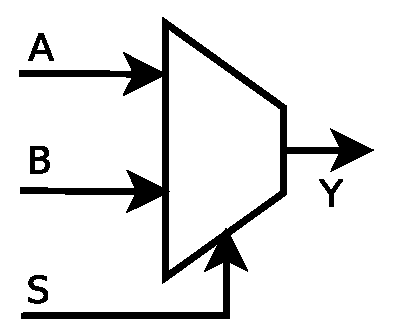
\includegraphics[width=0.7in]{images/mux.eps}
\caption{Multiplexer}
\label{img:multiplexer}
\end{figure}

Using boolean logic we can write

\begin{equation}
\label{eq:boolean mux}
  y = A\neg S + BS
\end{equation}

When $A, B, S \in \mathbb{R}$ and $S \in \langle 0, 1 \rangle$ we can write nothing else than
\begin{equation}
\label{eq:fuzzy mux}
  y = A(1-S) + BS
\end{equation}

Other problem :
Consider simple two wheels robot, with four distance sensors, on figure \ref{img:robot}.
We can define robot state by following vector $R(n) = (r(n), l(n), \theta(n), s_0(n), s_1(n), s_2(n), s_3(n))$,
where \\
$r(n)$ is right motor input \\
$l(n)$ is left motor input \\
$\theta(n)$ is robot orientation angle \\
$s_0(n)$ is front obstacle distance sensor output \\
$s_1(n)$ is left obstacle distance sensor output \\
$s_2(n)$ is rear obstacle distance sensor output \\
$s_3(n)$ is left obstacle distance sensor output \\
\\
\begin{figure}[!ht]
\centering
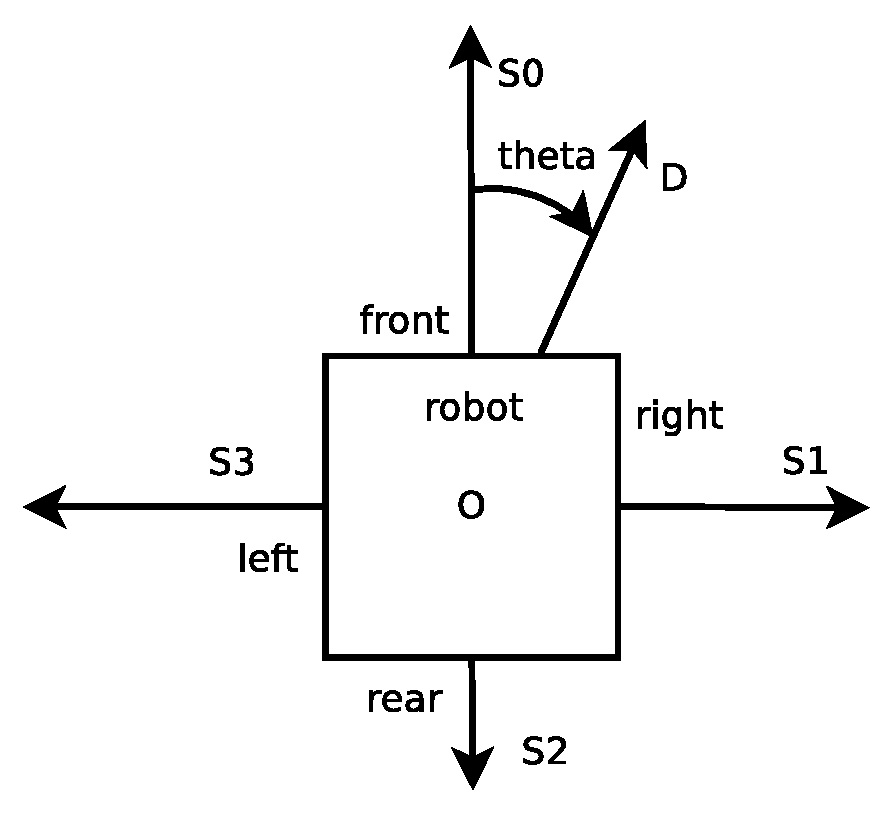
\includegraphics[width=1.8in]{images/robot.eps}
\caption{Robot}
\label{img:robot}
\end{figure}
\\
Our goal is determine prediction in G samples : $R(n+G)$. We can estimate exact physical model of robot and use it for modeling output (citovat tradicne modelovanie).
Simplified robot model can be written as rotation and moving.
 Situation for front sensor is describen in equation \ref{eq:exact_model}.
\\
\begin{align}
\label{eq:exact_model}
	s_0'(n) = min ( &D(n) + H(\theta(n))s_0(n) , \\
			&D(n) + H(\theta(n) + \frac{\pi}{2})s_1(n) , \nonumber \\
			&D(n) + H(\theta(n) + \pi s_2(n)) , \nonumber \\
			&D(n) + H(\theta(n) + \frac{3\pi}{2})s_3(n)) \nonumber
\end{align}
Where
$D(n)$ is robot position matrix, obtained from robots wheels speed. \\
$\theta(n)$ is rotation angle, calculated as speed diference of right and left motor $\theta(n) = b(r(n) - l(n))$ \\
$H(\theta(n))$ is rotation matrix for 2D vector around $\theta$ angle. \\
When different motors (wheels count, diameter, power, etc.) or sensors (count, range, angles, etc.) are used, we need to modify model. Biological systems are based on self model estimating (citovoat biological learning) and robustness (citovat napr Mark Tildena), using senses confrontation with their model citovat. This solution is robust and durable to system modification.

There is possible to use neural network (similar like biological systems) to create robot model.
We can see from \ref{eq:exact_model} there is not simple to process multiplicaiton with rotation vector using McCulloch Pitts neuron model.



\section{Neuron model}

We can simply solve proposed problems, adding multiplication matrix into neuron model

\begin{equation}
\label{eq:testing_neuron_1}
  y(n) = \varphi(\sum_{i = 0}^{N-1} x_i(n)w_i(n) + \sum_{j = 0}^{N-1} \sum_{i = j}^{N-1} x_j(n)x_i(n)v_{ji}(n))
\end{equation}

or more generally

\begin{equation}
\label{eq:testing_neuron_2}
  y(n) = \sum_{i = 0}^{N-1} x_i(n)w_i(n) + \sum_{j = 0}^{N-1} \sum_{i = j}^{N-1} x_j(n)x_i(n)v_{ji}(n) +  \sum_{j = 2}^{N-1} \sum_{i = 0}^{N-1} x_i^j(n)q_{ji}(n)
\end{equation}

where \\
$v(n)$ is matrix for two inputs multiplication \\
$q(n)$ is matrix for input power series multiplication \\

In \ref{eq:testing_neuron_2} we replace $\varphi(x)$ with power series
- this can be done beacuse of \cite{bib:taylor_01} and \cite{bib:taylor_02}.


\subsection{Neuron learning}

For basic learning, we can use gradient method.
We can define error as $e(n) = y_r(n) - y(n)$, where $y_r(n)$ is required output corresponding
to input $x(n)$.

Basic gradient learning can be written as
\begin{equation}
\label{eq:neuron_learning_1}
  w_i(n) =  w_i(n-1) + \eta e(n)x_i(n)
\end{equation}

Considering product $x_j(n)x_i(n)$ and $x_i^j(n)$ is nothing else than other input we can write for testing neuron

\begin{align}
\label{eq:neuron_learning_1}
  v_{ji}(n) &=  v_{ji}(n-1) + \eta e(n)x_j(n)x_i(n) \\
  q_{ji}(n) &=  q_{ji}(n-1) + \eta e(n)x_i^j(n)
\end{align}

To avoid local minima, some stochastic algorithm can be used - well know is simulated annealing.
First we need to define fitness function for all required outputs as

\begin{equation}
\label{eq:fitness}
  \lambda(n) = \lambda(n-1) + \sum_{i = 0}^{Y-1} e_i(n)^2
\end{equation}

and network parameters $N(n) \in \{\lambda(n), w(n), v(n), q(n)\}$.
We also mark best neural network as $N$ and some testing neural network as $N'$,
where $\lambda_N \leq \lambda_{N'}$
\begin{equation}
 N(n+1) =
  \begin{cases}
    N(n)' &  if \lambda_N' \le \lambda_{N} \lor pT(n) > rnd(0, 1)\\
    N(n)  &  otherwise\\
  \end{cases}
\end{equation}


\section{Experimental results}

In this part we describe our experimental results on function approximation ability.

\subsection{Testing functions}
Few function approximation tests were done - each experiment ID correspond to one
of testing function from \ref{eq:testing_functions}. We choose four categories of functions

\begin{itemize}
  \item Fuzzy logic - first three, using Łukasiewicz logic (citovat)
  \item Continuous nonlinear functions, with many multiplications
  \item Xor problem, with $sgn(x)$
  \item Four randomly initialized neural networks
\end{itemize}

Our goal was to cover principal approximation from spread set's of problems.

All functions have two inputs, in range $\langle -1, 1, \rangle$ and single output.
For correct neural network learning, one additional input was used as bias, with constant value $1.0$.

Last four testing functions were randomly initialized feed forward neural networks,
with different activation function's and different count of hidden layers $\langle 1, 3\rangle$, always with 32
neurons, with single output and three inputs - two for random input from $\langle 1, 3\rangle$ and one for bias.

\begin{align}
\label{eq:testing_functions}
  y &= \neg(x_0 \and x_1) \nonumber \\
  y &=  ((x_0 \and x_1) \lor x_1) \and \neg(x_0 \and x_1) \nonumber \\
  y &= x_0x_1 \nonumber \\
  y &= sin(5.0x_0 x_1) \nonumber \\
  y &=  0.25(cos(x_0x_1 + 0.731) - cos(2.3x_0 - 4.45x_1)  \nonumber \\
        &-cos(sin(3.17x_0 - 2.787x_1))sin(3.5435x_0)  \nonumber \\
        &+sin(x_1 + 5.0x_0x_1)) \nonumber \\
  y &= sin(3.3214x_0)sin(3.742x_1) \nonumber \\
  y &= sgn(x_0x_1) \nonumber \\
  y &= \frac{x_0 + x_1}{2.0} \nonumber \\
  y &= nn(linear, 1) \nonumber \\
  y &= nn(tanh, 1) \nonumber \\
  y &= nn(tanh, 2) \nonumber \\
  y &= nn(tanh, 3) \nonumber \\
\end{align}

\subsection{Neural network conditions}
Each neural network have some parameters, with difference only in neuron model type
and hidden layers count \ref{eq:nn_conditions}, \ref{eq:knn_conditions}. In our experiments,
these topology was testeted :
feed forward neural network's with 1 or 2 hidden layers, Kohonen network function approximation,
and finally feed forward neural network's with input preprocessing in Kohonen network.

Each network configuration had limited weight range, and output range $y_{max} \in \langle -1, 1 \rangle$.

\begin{align}
\label{eq:nn_conditions}
neuron\_type &= \{ \nonumber \\
                &NEURON\_TYPE\_LINEAR, \nonumber \\
                &NEURON\_TYPE\_TANH, \nonumber \\
                &NEURON\_TYPE\_TESTING \} \nonumber \\
init\_vector &= {see text} \nonumber \\
weight\_range &= 4.0 \nonumber \\
initv_weight\_range &= weight\_range/4 \nonumber \\
\eta &= 1.0/1000.0; \nonumber \\
y_{max} &= 4.0
\end{align}


\begin{align}
\label{eq:knn_conditions}
neurons\_count &= 8; \nonumber \\
weight\_range &= 1.0; \nonumber \\
\eta &= 1.0/100.0; \nonumber \\
y_{max} &= 1.0; \nonumber \\
\end{align}

\newpage
\subsection{Results}

Each network was tested on 12 different functions. And each function was running
16-teen times - trials, to show indenpendency from initial weight values. These
result can be seen on fig \ref{img:NN Trials run example}. We can see, only little average
results fluctuations.

\begin{figure}[!ht]
\centering
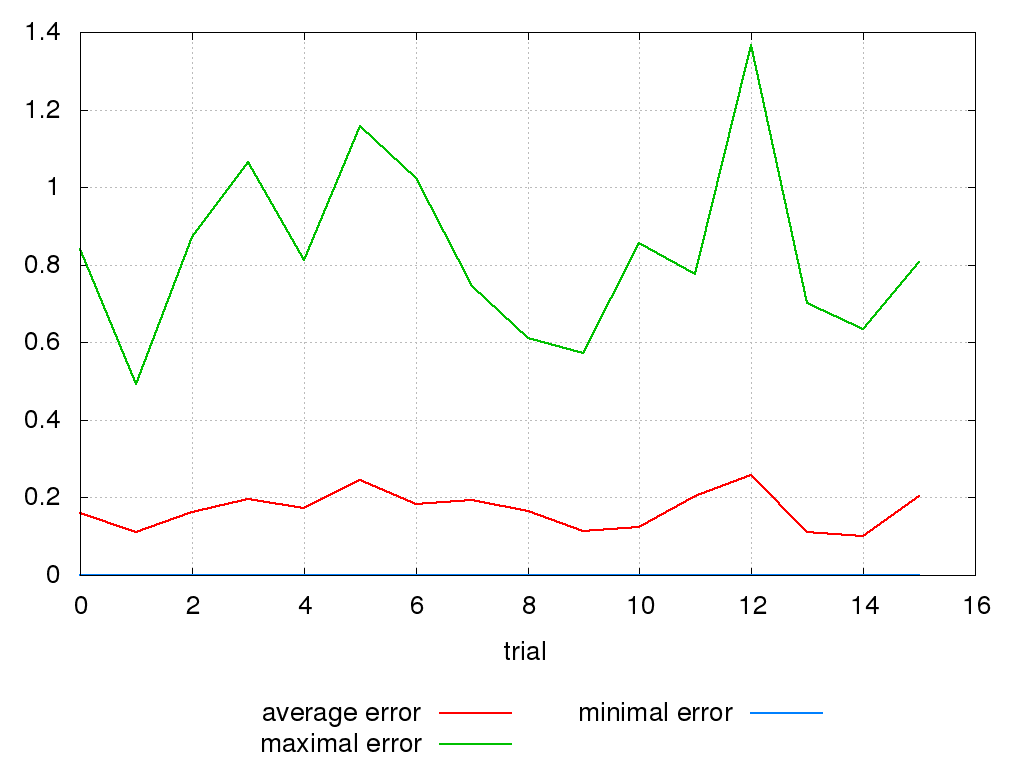
\includegraphics[width=3.5in]{images/error_log.png}
\caption{Trials run example}
\label{img:NN Trials run example}
\end{figure}

Summary results, for all network configurations, resulting averaging all 16 trials
can be seen on fig \ref{img:NN Average results}. Testing neuron with one hidden layer
configuration (cyan color) have in all experiments best error results. Second best
results achieved McCulloch-Pitts neuron with one hidden layers. For two hidden layers,
backpropagation learning algorithm have pure rusults in all cases - in next experiments is
necessary to use some stochastic optimization insted of backpropagation.

Partial results, for each experiment can be seen on figures \ref{img:mcculloch_pitts_tanh_neuron},
\ref{img:testing_neuron_1_layer_summary}, \ref{img:kohonen_layer_mcculloch_pitts_tanh_neuron_1_layer_summary},
\ref{img:kohonen_layer_testing_neuron_1_layer_summary}. Each of these figures represents different neuron
model, and is resulting minimum, maximum and average error for 16 trials for each approximating function.


\begin{figure}[!ht]
\centering
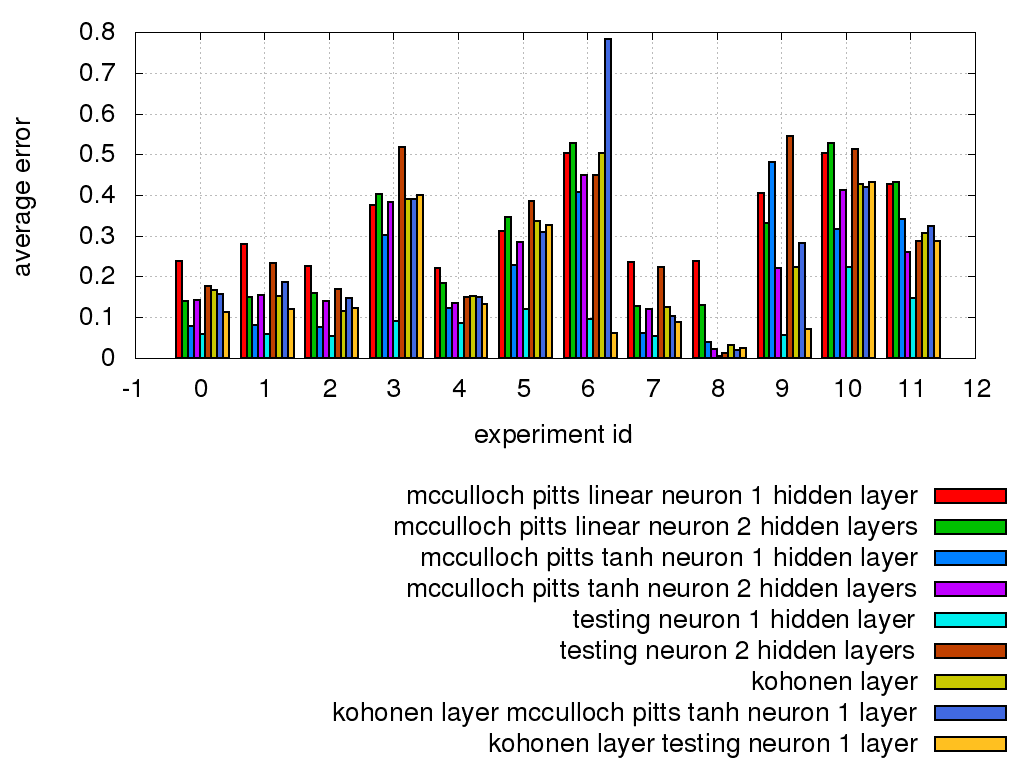
\includegraphics[width=4.5in]{images/summary_result_all_average_error_log.png}
\caption{Average results}
\label{img:NN Average results}
\end{figure}


\begin{figure}[!ht]
\centering
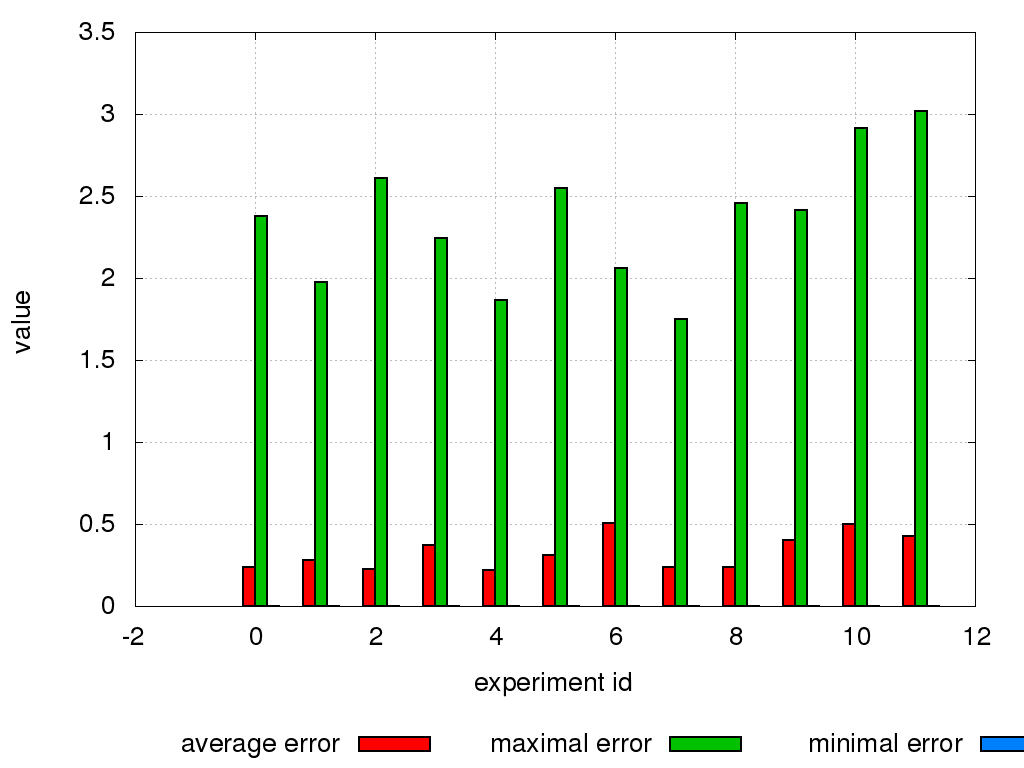
\includegraphics[width=4.0in]{images/mcculloch_pitts_tanh_neuron_1_layer_summary_result_log.png}
\caption{McCulloch-Pitts neuron with tanh activation function, single hidden layer}
\label{img:mcculloch_pitts_tanh_neuron}
\end{figure}

\begin{figure}[!ht]
\centering
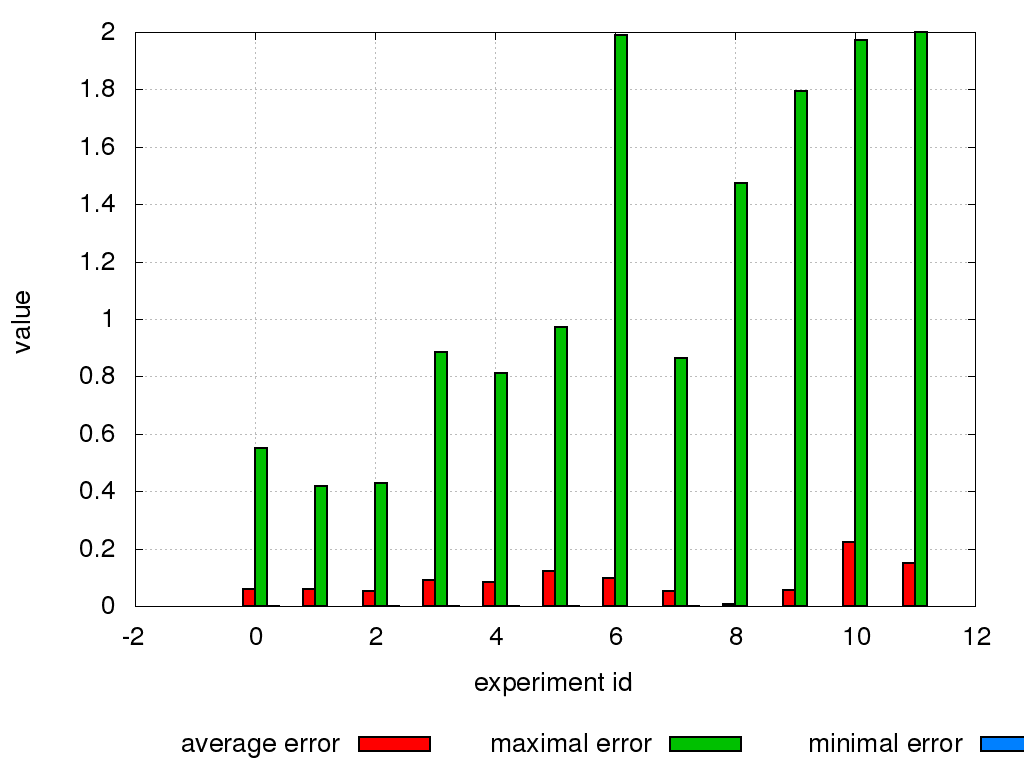
\includegraphics[width=4.0in]{images/testing_neuron_1_layer_summary_result_log.png}
\caption{Testing neuron with tanh activation function, single hidden layer}
\label{img:testing_neuron_1_layer_summary}
\end{figure}

\begin{figure}[!ht]
\centering
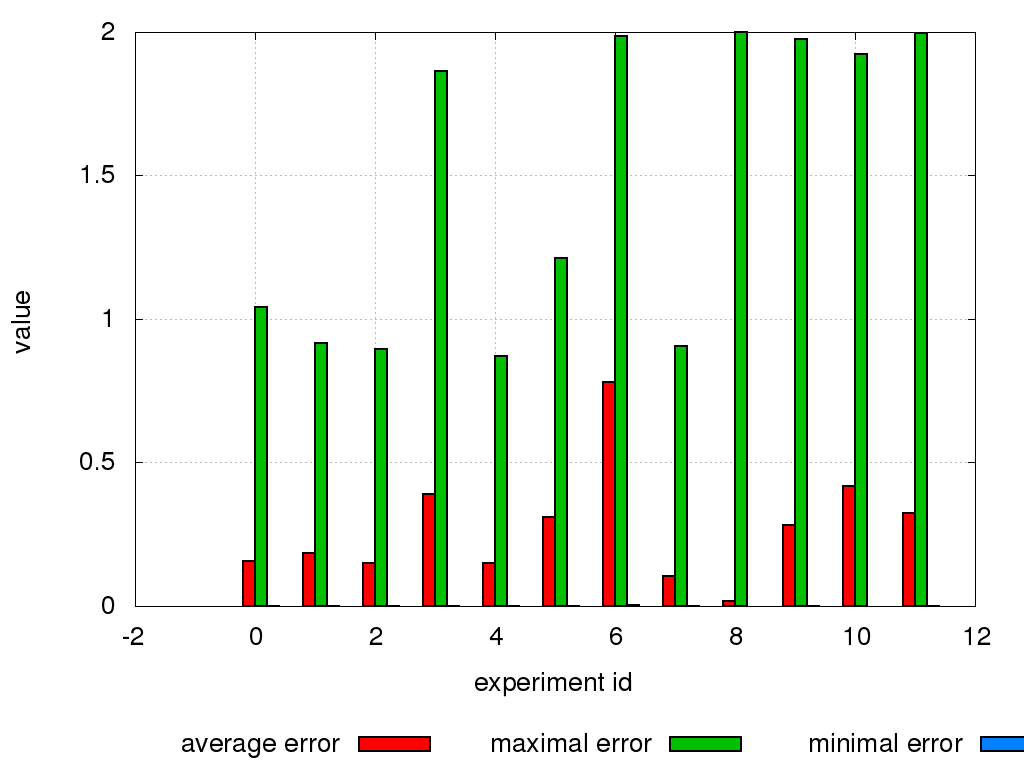
\includegraphics[width=4.0in]{images/kohonen_layer_mcculloch_pitts_tanh_neuron_1_layer_summary_result_log.png}
\caption{kohonen layer mcculloch pitts tanh neuron 1 layer summary}
\label{img:kohonen_layer_mcculloch_pitts_tanh_neuron_1_layer_summary}
\end{figure}

\begin{figure}[!ht]
\centering
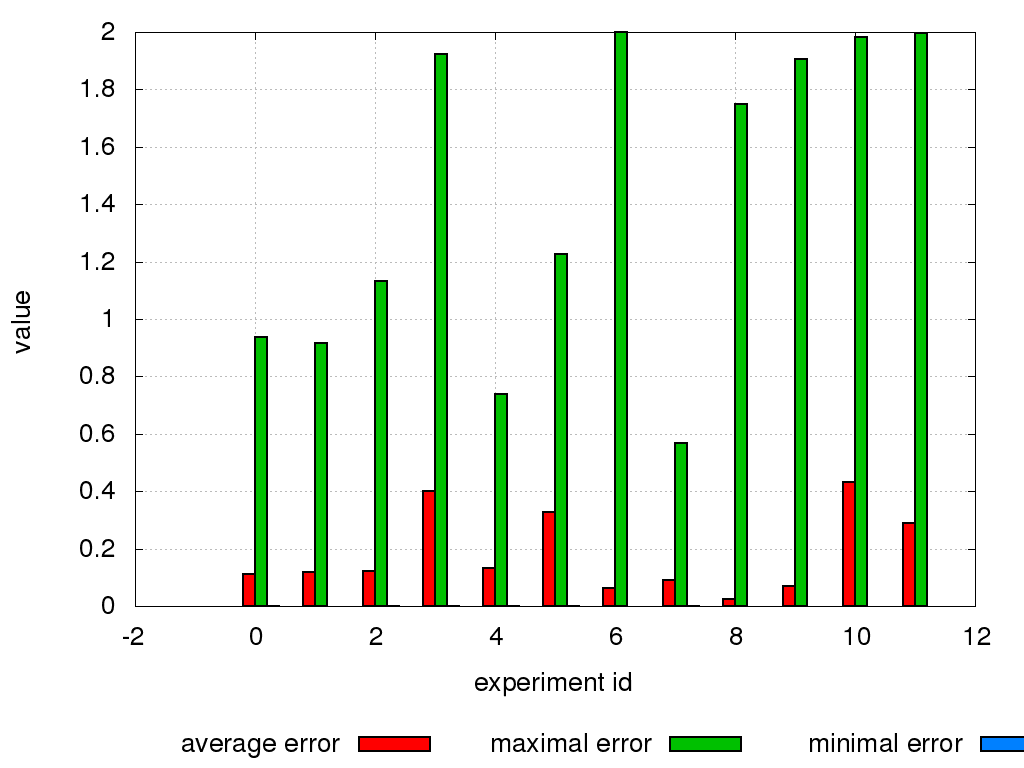
\includegraphics[width=4.0in]{images/kohonen_layer_testing_neuron_1_layer_summary_result_log.png}
\caption{kohonen layer testing neuron 1 layer summary}
\label{img:kohonen_layer_testing_neuron_1_layer_summary}
\end{figure}

\begin{figure}[!ht]
\centering
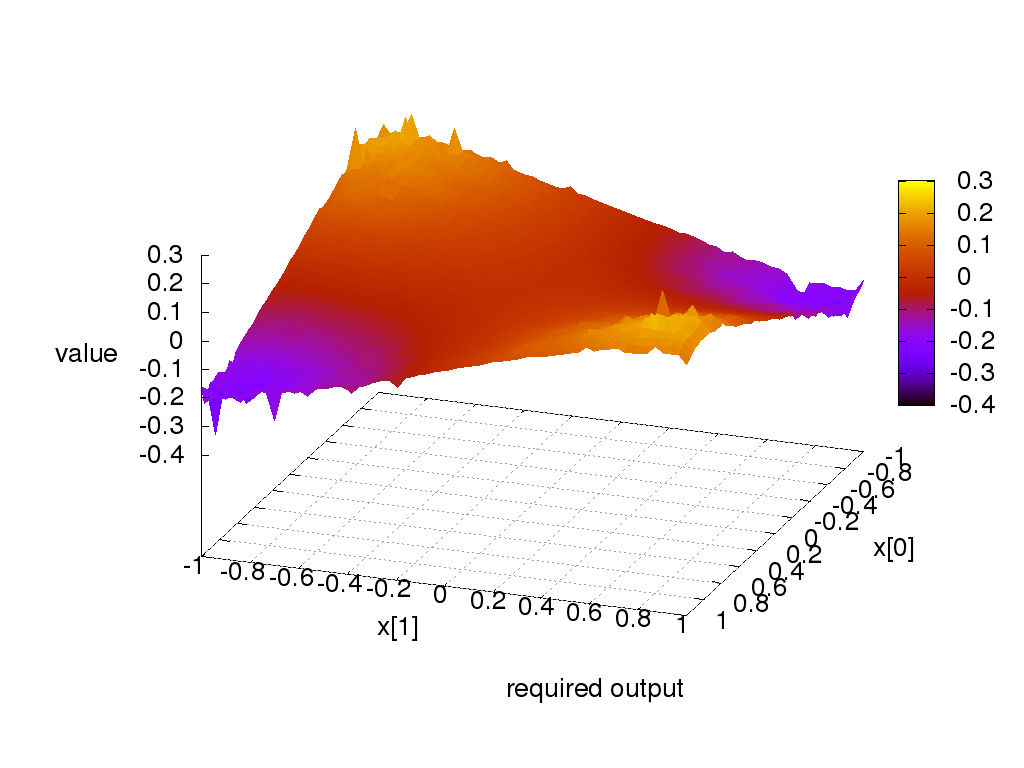
\includegraphics[width=4.0in]{images/result_log_required_output.png}
\caption{Required output example for experiment id 2}
\label{img:NN required output example for experiment id 2}
\end{figure}


\begin{figure}[!ht]
\centering
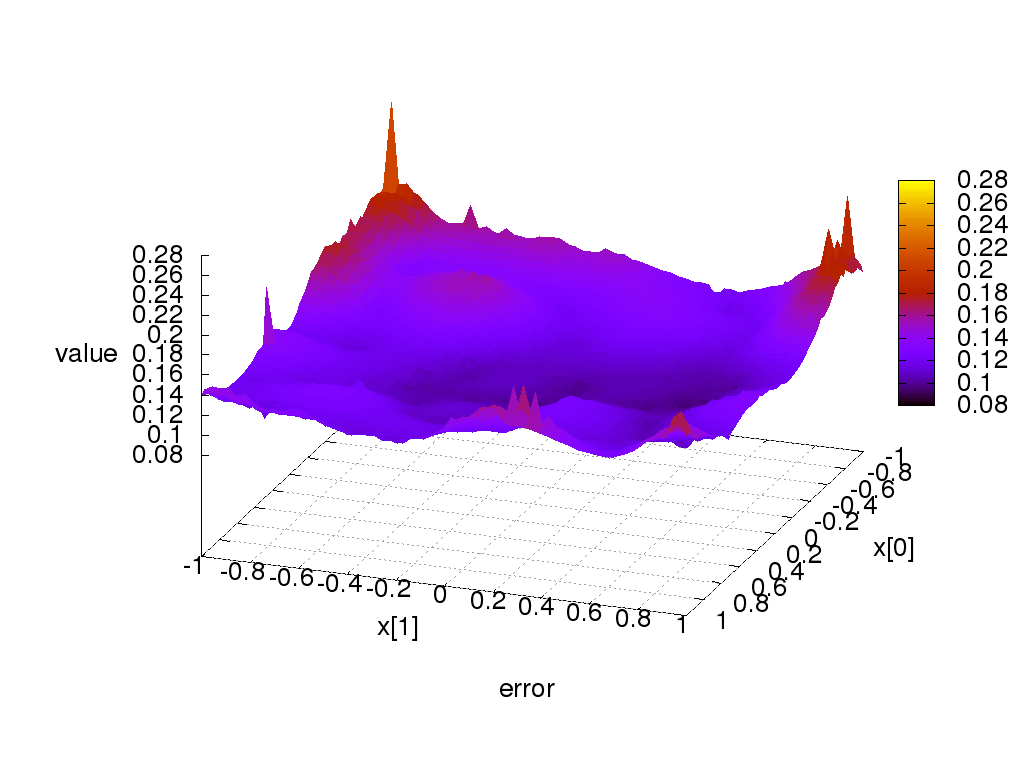
\includegraphics[width=4.0in]{images/mcculloch_pitts_tanh_neuron_1_layer_result_log_output_error.png}
\caption{Error surface for McCulloch-Pitts neuron for experiment id 2}
\label{img:NN error example 02}
\end{figure}


\begin{figure}[!ht]
\centering
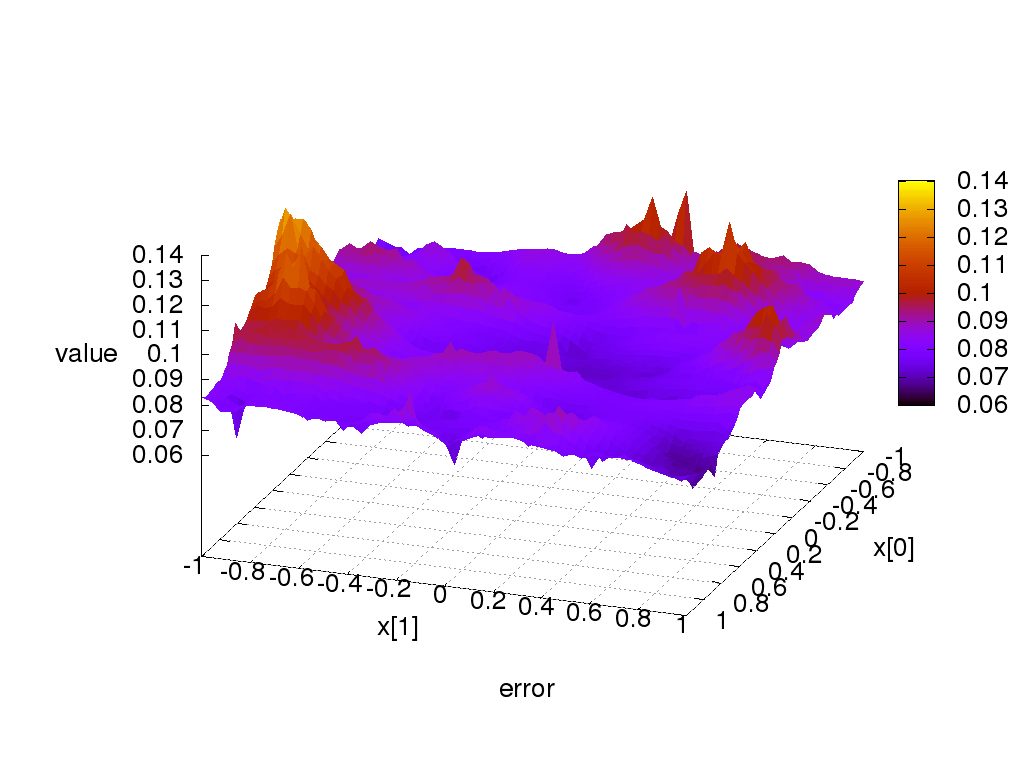
\includegraphics[width=4.0in]{images/testing_neuron_1_layer_result_log_output_error.png}
\caption{Error surface example for testing neuron for experiment id 2}
\label{img:NN error example 01}
\end{figure}

\subsection{Conclusion}

see ya

\bibliographystyle{IEEEtran}
\bibliography{bib}

\begin{thebibliography}{4}

\bibitem{bib:Approximation_1} Kolmogorov's Theorem,
http://neuron.eng.wayne.edu/tarek/MITbook/chap2/2\_3.html

\bibitem{bib:Approximation_2} Silvia Ferrari, Member, IEEE, and Robert F. Stengel, Fellow, IEEE, Smooth Function Approximation Using
Neural Networks, http://www.princeton.edu/~stengel/TNN2005.pdf

\bibitem{bib:Approximation_3} Yinyin Liu, Janusz A. Starzyk, Senior Member, IEEE, and Zhen Zhu, Member, IEEE,  Optimized Approximation Algorithm in Neural Networks Without Overfitting
http://www.ohio.edu/people/starzykj/network/research/Papers/Overfitting%20TNN06-P1314R%20manuscript.pdf

\bibitem{bib:Approximation_problem_1} Federico Girosi, Thomaso Poggio - Representation propherities of networks
http://cbcl.mit.edu/people/poggio/journals/girosi-poggio-NeuralComputation-1989.pdf

\bibitem{bib:Approximation_problem_2} Guang-Bin Huang, Senior Member, IEEE,  Qin-Yu Zhu, and  Chee-Kheong Siew, Member, IEEE -  Real-Time Learning Capability of Neural Networks
http://citeseerx.ist.psu.edu/viewdoc/download?doi=10.1.1.217.2612\&rep=rep1\&type=pdf

\bibitem{bib:Backpopagation_01} R. Rojas: Neural Networks, Springer-Verlag, Berlin, 1996 - R. Rojas: Neural Networks, Springer-Verlag, Berlin, 1996
http://page.mi.fu-berlin.de/rojas/neural/chapter/K7.pdf

\bibitem{bib:NN_Applications_01} neural network's applications
http://www.alyuda.com/products/forecaster/neural-network-applications.htm

\bibitem{bib:taylor_01} Taylor and Maclaurin Series
https://cims.nyu.edu/~kiryl/Calculus/Section\_8.7--Taylor\_and\_Maclaurin\_Series/Taylor\_and\_Maclaurin\_Series.pdf

\bibitem{bib:taylor_02} TAYLOR’S THEOREM
http://www.dcs.warwick.ac.uk/people/academic/Steve.Russ/cs131/NOTE26.PDF


\end{thebibliography}



\end{document}
